\documentclass[a4paper,12pt,nottoc]{article}
\usepackage{graphicx}
\usepackage[left = 3cm, right = 2cm, top = 2cm, bottom = 2cm]{geometry}
\usepackage{makecell}
\usepackage{booktabs}
\usepackage[justification=centering]{caption}
\usepackage{listings}
\usepackage{color}
\usepackage{xcolor}
%\usepackage{hyperref}
\usepackage{tocbibind}
\usepackage{amsmath}

\begin{document}

\begin{center}{\LARGE Detecting Fake News with Supervised Learning}\\\vspace{.5cm}Benjamin R. Perucco\\\vspace{.25cm}December 30, 2020\end{center}

\section{Definition}

\subsection{Project Overview}

Our world is highly interconnected and it is of paramount importance that citizens are informed objectively about issues that influence and shape our world (like issues on geopolitics or climate change). The internet lead to a rise of news media (e.g. social media, news portals, etc.) to report on these stories. The vast amount of (online) articles available yield a new phenomenon called fake news. Fake news is false or misleading information presented as news and can reduce the impact of real news \cite{bib:fakenews}. 

\subsection{Problem Statement}

This works' intention is about answering the question whether machine learning can be applied to classify a news article as truthful or fake. There are several articles available where Ahmed et al. classified news articles \cite{bib:ahmed-2017} or hotel guest reviews \cite{bib:ahmed-2018} to be truthful or fake. Ahmed et al. used natural language processing (NLP) models to transform text into a structured, mathematical representation and achieved accuracies of 92\% \cite{bib:ahmed-2017}.\\

\noindent Based on a set of features $\{f_{1}, f_{2}, f_{3}, ... \}$ extracted from news articles, a machine learning algorithm needs to be trained to find the relationship $\hat{\theta}$ between the a priori known classifiction of the news articles $y$ ($=0$ for truthful and $=1$ for fake) and the set of extracted features $\{f_{1}, f_{2}, f_{3}, ... \}$. The relation can be written as

\begin{gather}
\hat{y} =\hat{\theta}(X)
\end{gather}

\noindent where $\hat{y}$ is the predicted class label by the trained function $\hat{\theta}$ applied to a feature matrix $X$. $\hat{\theta}$ must be trained on available data, such that

\begin{gather}\label{eq:sse}
\sum_{i=1}^{n} \left(y - \hat{y} \right)^2
\end{gather}

\noindent is minimal. Here it is assumed that we have $n$ news articles where it is already known whether they are truthful or not. A first step to be worked on in this report is to answer how to extract a feature matrix $X$ from a set of texts (or documents). How reliable is the prediction of class labels on unseen news articles once the function $\hat{\theta}$ has been found.

\subsection{Metrics}

Equation \ref{eq:sse} is rather used for regression problems where the predicted output is a continuous variable. For classification problems like news article classification into a truthful ($= 0$) and a fake class ($= 1$), the accuracy is a better metric. This can be nicely demonstrated by the confusion matrix

\begin{gather}
\begin{bmatrix}
& 1 & 0 \\
1 & \textrm{TP} & \textrm{FP} \\
0 & \textrm{FN} & \textrm{TN}
\end{bmatrix}.
\end{gather}

\noindent The entries in the row indicate predicted classes and the entries in the columns represent the real classes. Furthermore, TP stands for true positives, TN for true negatives, FP for false positives and FN for false negatives. To asses the performance of $\hat{\theta}$, the accuracy $a$ is considered, which can be calculated as

\begin{gather}\label{eq:acc}
a = \frac{\textrm{TP} + \textrm{TN}}{\textrm{TP} + \textrm{TN} + \textrm{FN} + \textrm{FP}}.
\end{gather}

\section{Analysis}

\subsection{Algorithms and Techniques}

News articles must be converted into a structured, mathematical representation in order it can be used by machine learning techniques. The following chapters disucss how we can convert text into numerical features.

\subsubsection{n-gram Model}

The $n$-gram is usually defined a contiguous sequence of words with length $n$. For example, if $n = 1$, we speak of a unigram that contains only single word tokens. Or if $n = 2$, we denote this as a bigram which is built on two adjacent word tokens.\\

\noindent Consider the following text: ``Sometimes we eat green apples, and sometimes, the apples we eat are red.'' Based on a unigram (1-gram), we obtain a set of tokens: $\{$'sometimes', `we', `eat', `apples', `green', `and', `the', `are', `red'$\}$. We can derive a frequency array of tokens in the text: [2, 2, 2, 2, 1, 1, 1, 1, 1]. For the bigram (2-gram), another set of tokens is obtained: $\{$'sometimes we', `we eat', `eat green', `green apples', `apples and', `and sometimes', `sometimes the', `the apples', `apples we', `eat are', `are red'$\}$. The corresponding frequency array of tokens in the text is: [1, 1, 1, 1, 1, 1, 1, 1, 1, 1, 1]. Please note that punctuation is not considered when converting text into tokens.\\

\noindent In order to build frequency arrays for a set of texts (or documents), a common vocabulary needs to be built of which the $n$-gram model is underlying principle.

\subsubsection{Vocabulary}

Consider a corpus $D$ which contains a set of documents $\{d_1, d_2, d_3, ..., d_n\}$. Then a vocubulary $F$ is a set of tokens $\{f_1, f_2, f_3, ..., f_m\}$ extracted from the corpus $D$. Please remind yourself that a token is created based on the n-gram model. Usually for a set of tokens, only the $m$ mostly occuring tokens in a corpus $D$ are considered. In the following, the tokens are denoted as features as these construct the features (or independent variables) of a machine learning model.\\

\subsubsection{Definitions}

Let $\sigma(d_i, f_j)$ denote the number of occurances of feature $f_j$ in document $d_i$. Then a feature matrix $S$ can be built, where

\begin{gather}
S =
\begin{bmatrix}
\sigma(d_1, f_1) & \sigma(d_1, f_2) & \sigma(d_1, f_3) & ... & \sigma(d_1, f_m) \\
\sigma(d_2, f_1) & \sigma(d_2, f_2) & \sigma(d_2, f_3) & ... & \sigma(d_2, f_m) \\
\sigma(d_3, f_1) & \sigma(d_3, f_2) & \sigma(d_3, f_3) & ... & \sigma(d_3, f_m) \\
... & ... & ... & ... & ... & \\
 \sigma(d_n, f_1) & \sigma(d_n, f_2) & \sigma(d_n, f_3) & ... & \sigma(d_n, f_m)
\end{bmatrix}.
\end{gather}

\noindent An element $\sigma(d_i, f_j)$ in matrix $S$ (representing the document $d_i$ and feature $f_j$) is abbreviated using the notation $\sigma_{ij}$ for simplicity.

\subsubsection{Term Frequency Model}

The matrix $S$ could be already used for machine learning. Features usually need to be normalized in machine learning to increase performance. Therefore, the term frequency (TF) model normalizes matrix $S$ leading to matrix $\hat{S}$. An element $\hat{\sigma}_{ij}$ of matrix $\hat{S}$ is written as

\begin{gather}\label{eq:tf}
\hat{\sigma}_{ij} = \frac{\sigma_{ij}}{\sum_{j=1}^{m}\sigma_{ij}}.
\end{gather}

\noindent Or spoken in plain language: the number of occurances of a token $f_j$ in a document $d_i$ is divided by the total number of occurances of all tokens $\{f_1, f_2, f_3, ..., f_m\}$ in the same document $d_i$. So we end up with a representation where the importance of each feature can be compared to other features in the same document.

\subsubsection{Inverse Document Frequency Model}

The inverse document frequency (IDF) model is used to define the feature importance not just in a document $d_i$ but also compare its importance within a corpus $D$. A matrix $E$ is introduced, where an element $\epsilon_{ij}$ of matrix $E$ is $1$ if $\hat{\sigma}_{ij} > 0$ (or $\sigma_{ij} > 0$). An inverse normalization is applied to the matrix $E$ resulting in a vector $\hat{e}$. An element $\hat{\epsilon}_{j}$ of vector $\hat{e}$ is calculated as

\begin{gather}\label{eq:idf}
\hat{\epsilon}_{j} = 1 + \textrm{log}\left[\frac{|D|}{\sum_{i=1}^{n}\epsilon_{ij}}\right].
\end{gather}

\noindent Or spoken in plain language: in a corpus $D$ which comprises of a set of documents $\{d_1, d_2, d_3, ..., d_n\}$, it is counted in how many documents the feature $f_j$ appears. This number is used to divide the number of documents $|D|$ in a corpus $D$. Consider two examples: if a feature $f_j$ occurs in each document $\{d_1, d_2, d_3, ..., d_n\}$, we divide the number of documents $|D|$ in a corpus $D$ by the same number. So equation \ref{eq:idf} results in $1$, weighting feature $f_j$ as $1$. On the other hand, if a feature $f_j$ occurs only in one document, equation \ref{eq:idf} produces a much larger number, thus increasing the weight of feature $f_j$ in the corpus $D$.\\

\noindent Finally, a matrix $\hat{P}$ is obtained as the element-wise product of the term frequency matrix $\hat{S}$ and the inverse document frequency vector $\hat{e}$, written as $\hat{P} = \hat{S} \odot \hat{e}$. For an element $\hat{\pi}_{ij}$ of matrix $\hat{P}$, this is written as

\begin{gather}\label{eq:tf-idf}
\hat{\pi}_{ij} = \hat{\sigma}_{ij} \cdot \hat{\epsilon}_{j},\;\;\textrm{element-wise for}\;j = 1, 2, 3, ..., m .
\end{gather}

\noindent This term is denoted as the term frequency inverse document frequency model (TF-IDF).

\subsection{Data Exploration}

A set of truthful and fake news articles is available on kaggle.com \cite{bib:kaggle}. The data was collected from real world sources. Truthful articles were obtained from Reuters and fake news articles were gathered from unreliable websites that were flagged by Politifact which is a fact-checking organization. These datasets contain different types of articles on different topics, the majority of articles focus on political and world news topics \cite{bib:ahmed-2018}.\\

\noindent There are 44,898 articles in total in the corpus. 21,417 of the articles are classified as truthful and 23,481 are classified as fake, so both class labels are roughly balanced. Approximately 6,169 of the articles are not unique. The duplicates are being removed after text processing discussed in chapter \ref{chap:data-preproc}.

\subsubsection{Visual Analysis of Top Features}

A first glimpse of the top 20 unigrams per class is given in figure \ref{fig:top20}. Please note that the extracted unigrams are based on the processed text. It can be observed from the unigrams that probably the most discussed topic in the set of news articles is the presidential election in the U.S. during the year 2016. Despite some unigrams that are used frequently in both classes of articles (like said, trump, presid, republican, etc.), we also see distinct unigrams only used in one class of articles.

\begin{figure}[h]
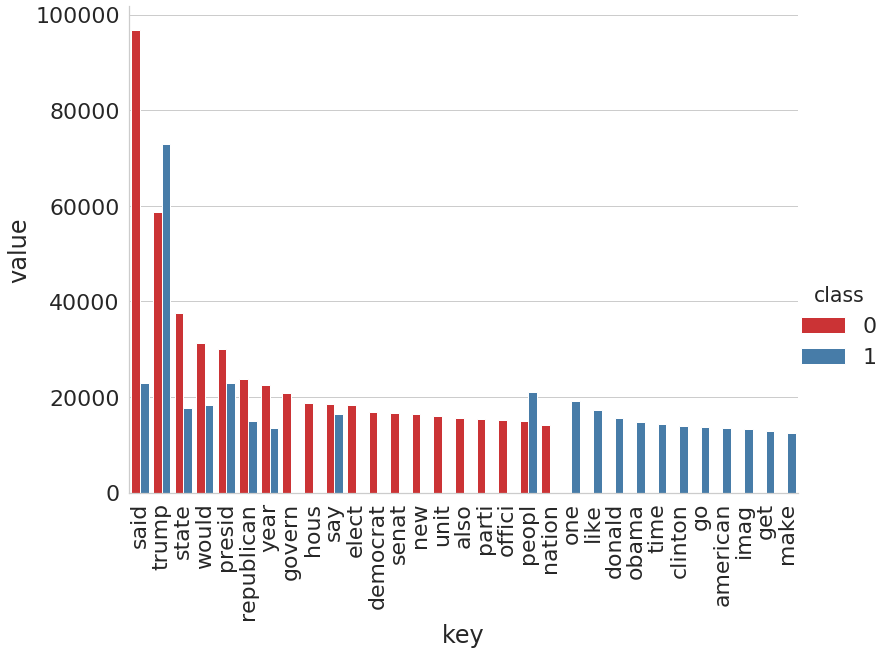
\includegraphics[width=14cm]{output/word_analysis_1.png}
\centering
\caption{Frequency of the top 20 unigrams per class extracted from the corpus.}\label{fig:top20}
\end{figure}

\section{Methodology}

\subsection{Data Preprocessing}\label{chap:data-preproc}

Raw text has to be brought into a clean state in order for feature extraction. Several text cleansing steps are performed like removal of introductory statements, dates, hyperlinks, numbers and stopwords. Finally, so called stemming is performed to end up with the stem of a word (for example cat should identify such strings as cats, catlike, and catty \cite{bib:stemming}).

\subsection{Implementation}

\subsubsection{Feature Extraction Method}

Then the randomized corpus is split into three different datasets as displayed in the table below.

\begin{center}
\begin{tabular}{| l | l | r | c | c | c |}
\hline
Name & Purpose & Size & TF & IDF & TF-IDF \\
\hline
Training & Model training & 60\% & $\hat{S}_{\textrm{train}}$ & $\hat{E}_{\textrm{train}}$ & $\hat{S}_{\textrm{train}} \odot \hat{E}_{\textrm{train}}$ \\  
Test & Hyperparameter tuning & 20\% & $\hat{S}_{\textrm{test}}$ & $\hat{E}_{\textrm{train}}$ & $\hat{S}_{\textrm{test}} \odot \hat{E}_{\textrm{train}}$ \\    
Validation & Model validation & 20\% & $\hat{S}_{\textrm{valid}}$ & $\hat{E}_{\textrm{train}}$ & $\hat{S}_{\textrm{valid}} \odot \hat{E}_{\textrm{train}}$ \\
\hline 
\end{tabular}
\end{center}

\noindent It is good practise not to use the same data for model training and validation. For hyperparameter tuning a test dataset is used to avoid overfitting.\\

\noindent Term frequency (TF) feature matrices are calculated for each set according to equation \ref{eq:tf}. In comparison, the inverse document frequency (IDF) feature matrix is only calculated for the training set according to equation \ref{eq:idf}. The reason is that the validation and test set should simulate the performance behaviour in case of new unseen data. Therefore,  the IDF feature matrix is estimated on a hypothetical training set and the resulting matrix $\hat{E}_{\textrm{train}}$ is used for the transformation of all sets into the TF-IDF feature space according to equation \ref{eq:tf-idf}. Contrary, the TF feature matrix describes the relative importance of features in a single document. This is independent of other documents in the corpus and therefore, we can derive three matrices $\hat{S}_{\textrm{train}}$, $\hat{S}_{\textrm{test}}$ and $\hat{S}_{\textrm{valid}}$ for the three sets.

\subsubsection{Modeling}

\noindent SageMaker \cite{bib:sagemaker} is used as the training and deployment platform for the machine learning models. The evaluated machine learning models are based on the sci-kit learn framework \cite{bib:scikit-learn} because of its simplicity to try out different machine learning models.\\

\noindent The following models k nearest neighbor (knn), support vector machine (svm), logistic regression (log), gradient boosting (gbc) and multilayer perceptron (mlp) are used. Furthermore, the TF and TF-IDF feature extraction methods are applied. The feature size is set to 500, 1000 and 5000 features and unigram and bigram are used for feature extraction.

\subsection{Refinement}

Hyperparameter tuning is performed on the training set and tested on the test set according to the accuracy (equation \ref{eq:acc}). A hyperparameter set is search for which maximizes the accuracy. For the hyperparameter search, 20 combinations are evaluted and in total this results in 1200 models to be trained and tested (5 models x 2 feature extraction methods x 3 different feature sizes x 2 differnt n-grams x 20 models for hyperparameter tuning). In the following table \ref{tab:hyperparam}, the model hyperparameters as well as its varied ranges are shown. 

\begin{table}[h]
\begin{center}
\begin{tabular}{| l | l | l |}
\hline
Parameter & Type & Range \\
\hline
\multicolumn{3}{| c |}{k nearest neighbor \cite{bib:knn}} \\ [.1cm]
\hline
n neighbors & int & [3, 15] \\
weight & cat & 'uniform', 'distance'\\
p & int & [1, 8] \\
\hline 
\multicolumn{3}{| c |}{support vector machine \cite{bib:svm}} \\ [.1cm]
\hline
random state & int & 1 \\
kernel & cat & `poly' \\
C & float & [0.001, 3.0] \\
degree & int & [2, 3] \\
\hline 
\multicolumn{3}{| c |}{logistic regression \cite{bib:log}} \\ [.1cm]
\hline
max iter & int & 10,000 \\
C & float & [0.001, 3.0] \\
\hline
\multicolumn{3}{| c |}{gradient boosting \cite{bib:gbc}} \\ [.1cm]
\hline
random state & int & 1	 \\
learning rate & float & [0.001, 0.5] \\
n estimators & int & [100, 1000] \\
max depth & int & [2, 10] \\
\hline 
\multicolumn{3}{| c |}{multilayer perceptron \cite{bib:mlp}} \\ [.1cm]
\hline
random state & int & 1	 \\
learning rate & float & [0.0001, 0.1] \\
max iter & int & [100, 10000] \\
activation & cat & 'identity', 'logistic', 'relu', 'tanh' \\
hidden layer size & int & [2, 10] \\
start size$^\textrm{1}$ & int & [10, 1000] \\
end size$^\textrm{1}$ & int & [10, 1000] \\
\hline
\end{tabular}
\caption{$^\textrm{1}$ Note that start and end size are not available as parameters in the multilayer perceptron model in scikit-learn. Based on the hidden layer size and its start and end size, a linear interpoliation is performed for the number of neurons in between in case the hidden layer size is higher than 2.}\label{tab:hyperparam}
\end{center}
\end{table}

\section{Results}

\subsection{Model Evaluation and Validation}

\subsubsection{Top 5 Accuracy Performance}

\subsubsection{Influence of Parameter Variation}

In total there are 60 parameter variations studied (5 models x 2 feature extraction methods x 3 different feature sizes x 2 differnt n-grams). Per parameter combination, the model is taken which leads in the highest accuracy after hyperparameter tuning. The influence of the different parameters is demonstrated below. In figure \ref{fig:modelperf}, the model performance can be seen for the five machine learning models evaluated. 

\begin{figure}[h]
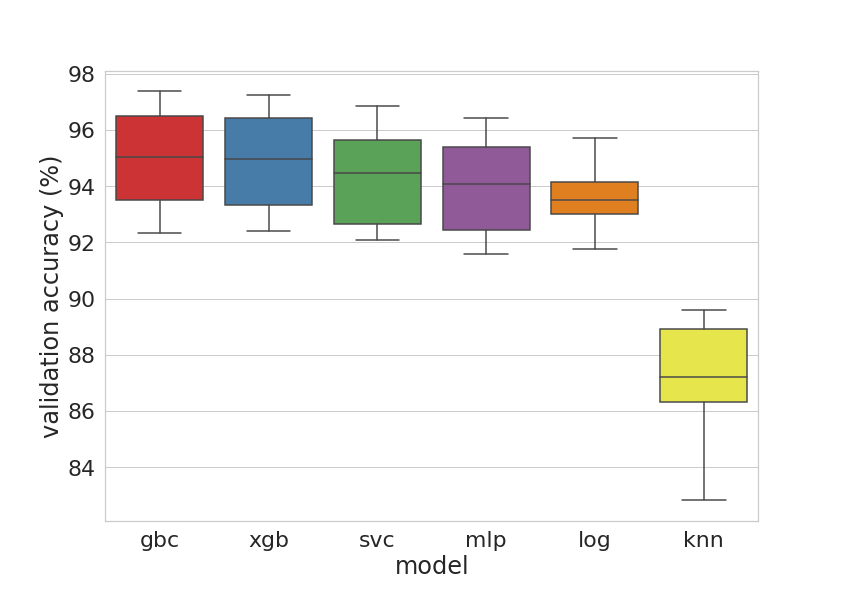
\includegraphics[width=14cm]{output/model_performance.png}
\centering
\caption{Model performance of five evaluated machine learning models.}\label{fig:modelperf}
\end{figure}

\subsection{Justification}

\section{Conclusion}

\subsection{Reflection}

\subsection{Improvement}



%\section*{Domain Background}
%
%Our world is highly interconnected and it is of paramount importance that citizens are informed objectively about issues that influence and shape our world (like issues on geopolitics or climate change). The internet lead to a rise of news media (e.g. social media, news portal, etc.) to report on these stories. The vast amount of (online) articles available yield a new phenomenon called fake news. Fake news is false or misleading information presented as news and can reduce the impact of real news \cite{bib:fakenews}.
%
%\section*{Problem Statement}
%
%How can fake news be distingiushed from reliable and trustworthy information? In the following capstone project, a machine learning model shall be developed whose aim is to detect fake news. The underlying problem is to bring words and sentences into a mathematical representation for machine learning to be applied.
%
%\section*{Datasets and Inputs}
%
%Articles classified as fake and real news are needed in order to train machine learning models. Such a dataset is taken from kaggle \cite{bib:kaggle} and was collected from real world sources. Truthful articles were obtained from Reuters and fake news articles were gathered from unreliable websites that were flagged by Politifact which is a fact-checking organization. These datasets contain different types of articles on different topics, the majority of articles focus on political and world news topics \cite{bib:isot}, \cite{bib:ahmed-2018}, \cite{bib:ahmed-2017}. There are about 21,417 real news articles and about 23,481 fake news articles in the dataset. So data is roughly balanced. Furthermore, the data consists of four columns: title, text, subject and date.
%
%\section*{Solution Statement}
%
%Natural language processing (NLP) models are used to bring words and sentences into a mathematical representation. Often applied is the n-gram model which is a contiguous sequence of items with length $n$ (such as words or characters) to be analyzed. Based on the n-gram model, features can be extracted as discussed by Hadeer et al. \cite{bib:ahmed-2018}:
% 
% \begin{itemize}
%\item{Term frequency (TF): TF defines the number of times a words appears in a document with respect to the number of total words in the document.}
%\item{Term frequency-inverted document frequency (TF-IDF): TF-IDF is a statistical metric used to measure how important a term is to a document compared to a set of documents.}
%\end{itemize}
%
%\section*{Benchmark Model}
%
%Hadeer et al. \cite{bib:ahmed-2017} achieved an accuracy of 92 \% when a linear support vector machine (LSVM) combined with 1-gram model and a 50,000 top feature selection TF-IDF method was used.
%
%\section*{Evaluation Metrics}
%
%The evaluation metric for this formulated problem is accuracy. This means how many labels are correctly classified (either as fake or real news) in respect to all classified labels.
%
%\section*{Project Design}
%
%Machine learning models shall be developed on AWS SageMaker \cite{bib:sagemaker}. The following project design is proposed:
%
%\begin{itemize}
%\item{Article exploration: The nature of the articles is investigated and a text processing strategy is derived.}
%\item{Text processing: Articles need to be processed with respect to formation, stop word removal, stemming, etc.}
%\item{Feature extraction: Dictionaries and n-gram models are built and together with techniques such as TF and TF-IDF features are extracted.}
%\item{Data preparation: Training, test and validation data for the machine learning models are prepared, for example 60 \% training,  20 \% test and 20 \% validation data.}
%\item{Modeling: Four machine learning models are evaluated sourcing from different frameworks such as support vector machine (SVM) from scikit-learn, linear learner (LL) and xgboost (XGB) from SageMaker built-in models and recurrent neural network (RNN) based on PyTorch.}
%\item{Tuning and validation: The test data is used to tune the machine learning hyperparameters and the validation data is used to evaluate the final metrics and to clarify the best modeling strategy.}
%\end{itemize}
%
\begin{thebibliography}{9}
\bibitem{bib:fakenews} Fake news, December 30, 2020, wikipedia.org, \\\texttt{https://en.wikipedia.org/wiki/Fake\_news}
\bibitem{bib:ahmed-2017} Ahmed H., Traore I., Saad S. (2017) Detection of Online Fake News Using N-Gram Analysis and Machine Learning Techniques. In: Traore I., Woungang I., Awad A. (eds) Intelligent, Secure, and Dependable Systems in Distributed and Cloud Environments. ISDDC 2017. Lecture Notes in Computer Science, vol 10618. Springer, Cham. \texttt{https://doi.org/10.1007/978-3-319-69155-8\_9}
\bibitem{bib:ahmed-2018} Ahmed, H, Traore, I, Saad, S. Detecting opinion spams and fake news using text classification, Security and Privacy, 2018, \texttt{https://doi.org/10.1001/spy2.9}
\bibitem{bib:kaggle} Fake and real news dataset, December 30, 2020, kaggle.com, \\\texttt{https://www.kaggle.com/clmentbisaillon/fake-and-real-news-dataset}
\bibitem{bib:stemming} Stemming, December 30, 2020, wikipedia.org, \\\texttt{https://en.wikipedia.org/wiki/Stemming}
\bibitem{bib:sagemaker} Amazon SageMaker, December 30, 2020, amazon.com, \\\texttt{https://aws.amazon.com/sagemaker}
\bibitem{bib:scikit-learn} scikit-learn - machine learning in Python, December 30, 2020, scikit-learn.org, \\\texttt{https://scikit-learn.org/stable}
\bibitem{bib:knn} scikit-learn - classifier implementing the k-nearest neighbors vote, December 30, 2020, scikit-learn.org, \texttt{https://scikit-learn.org/stable/modules/generated/\\sklearn.neighbors.KNeighborsClassifier.html}
\bibitem{bib:svm} scikit-learn - c-support vector classification, December 30, 2020, scikit-learn.org, \texttt{https://scikit-learn.org/stable/modules/generated/\\sklearn.svm.SVC.html}
\bibitem{bib:log} scikit-learn - logistic regression classifier, December 30, 2020, scikit-learn.org, \texttt{https://scikit-learn.org/stable/modules/generated/\\sklearn.linear\_model.LogisticRegression.html}
\bibitem{bib:gbc} scikit-learn - gradient boosting for classification, December 30, 2020, scikit-learn.org, \texttt{https://scikit-learn.org/stable/modules/generated/\\sklearn.ensemble.GradientBoostingClassifier.html}
\bibitem{bib:mlp} scikit-learn - multilayer perceptron classifier, December 30, 2020, scikit-learn.org, \texttt{https://scikit-learn.org/stable/modules/generated/\\sklearn.neural\_network.MLPClassifier.html}
\end{thebibliography}

\end{document}